\problemname{Australian open}


\begin{figure}[!h]
\begin{center}
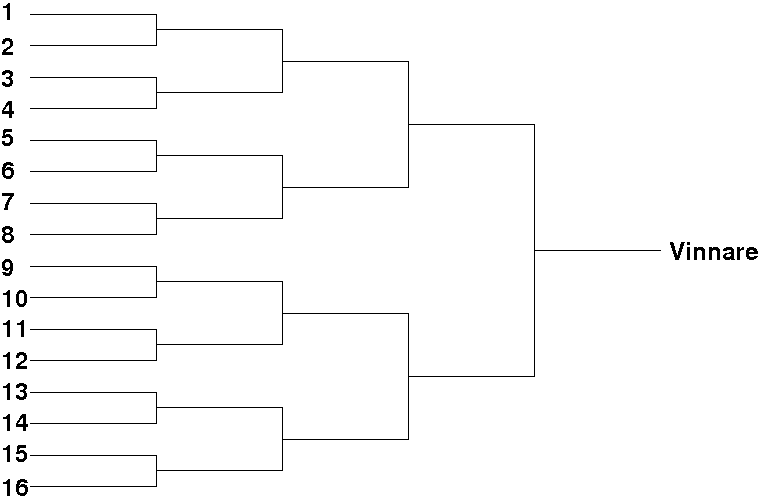
\includegraphics[width=0.5\textwidth]{australian.png}
\end{center}
\end{figure}

Årets stora idrottshändelse i Australien är naturligtvis International Olympiad in Informatics. I väntan på denna har man dock anordnat vissa sidoevenemang, exempelvis tennisturneringen Australian open. Detta är en {\em utslagsturnering} som kan
beskrivas med ett spelschema enligt figuren ovan, där antalet {\em omgångar} $n$ kan variera. Man startar alltså till vänster med $2^n$ spelare, numrerade från 1 till $2^n$. Efter totalt $2^n - 1$ matcher har man utsett en vinnare.

Vi antar nu att varje spelare $i$ har en ``förmåga'' $x_i$, och att när två spelare $i$ och $j$ möts, så vinner spelare $i$ med sannolikheten
\begin{displaymath}
P(i \text{ besegrar } j) = \frac{1}{1+\exp(x_j-x_i)}
\end{displaymath}
och annars vinner spelare $j$ eftersom en tennismatch inte kan sluta
oavgjort ($\exp(x)$ betecknar exponentialfunktionen $e^x$). Formeln är vald så att $P(i \text{ besegrar } j)+P(j \text{ besegrar } i)=1$.

Skriv ett program som, givet alla spelares förmågor, avgör vem som har
störst chans att vinna turneringen och hur stor denna chans är.


\section*{Indata}
På första raden står ett heltal $n$ ($1 \leq n \leq 10$), antal omgångar.
På andra raden står $2^n$ flyttal mellan 0 och 10, förmågan för
varje spelare i nummerordning.

\section*{Utdata}
Skriv ut ett heltal och ett flyttal: numret på den spelare som har
störst chans att vinna turneringen samt sannolikheten att den spelaren
vinner. Om flera spelare har störst chans kan du ange vilken som helst
av dem. Svaret accepteras om det absoluta felet är mindre än $10^{-5}$.

\noindent
\begin{tabular}{| l | l | p{12cm} |}
  \hline
  \textbf{Grupp} & \textbf{Poäng} & \textbf{Gränser} \\ \hline
  $1$    & $20$       & $n=1$ \\ \hline
  $2$    & $80$       & Inga ytterligare begränsningar. \\ \hline
\end{tabular}

\section*{Förklaring exempelfall 1}
Första matchen vinner spelare 1 med sannolikheten 0.549834 och spelare 2 med sannolikheten 0.450166.
Andra matchen vinner spelare 3 med sannolikheten 0.689974 och spelare 4 med sannolikheten 0.310026.
Dessa händelser är oberoende och därmed kan vi räkna ut sannolikheten
för varje möjligt finalpar genom att multiplicera sannolikheterna med
varandra. Det ger upphov till följande tabell:

\begin{tabular}{|c|c|c|c|c|c|c|} \hline
 & {\bf Sannolikhet att} & {\bf Sannolikhet att} & \multicolumn{4}{|c|}{\bf Bidrag till total chans att spelaren vinner}  \\
{\bf Match} & {\bf matchen spelas} & {\bf vinna matchen} & {\bf
  1}&{\bf 2}&{\bf 3}&{\bf 4} \\ \hline
1--3 & 0.379371 & 0.524979--0.475021 & 0.199162 & -- & 0.180209 & -- \\
1--4 & 0.170463 & 0.710950--0.289050 & 0.121190 & -- & -- & 0.049272 \\
2--3 & 0.310603 & 0.475021--0.524979 & -- & 0.147543 & 0.163060 & -- \\
2--4 & 0.139563 & 0.668188--0.331812 & -- & 0.093254 & -- & 0.046309 \\ \hline
{\bf Summa }& {\bf 1.000000} &                & {\bf 0.320352} & {\bf 0.240797} & {\bf 0.343269 }& {\bf 0.095581 } \\ \hline
\end{tabular}
